\documentclass[
   % 9b temf, 3b cem?
   accentcolor=9b,
   boxstyle=boxed
   ]{tudasciposter}

% default
\usepackage[ngerman]{babel}
\usepackage{microtype}
\usepackage[autostyle]{csquotes}

% additional
\usepackage{amsmath}

\usepackage{tikz}
\usepackage{pgfplots}
\usepackage{pgfplotstable}
\pgfplotsset{compat=newest}
\usepgfplotslibrary{units}
\usepgfplotslibrary{groupplots}
% colormap name=tuda
\usepackage{tuda-pgfplots}

\begin{document}
\title{Shape Optimization of a Compact DC Photo-Electron Gun using Isogeometric Analysis}
\author{Peter Förster$\mathbf{^1}$, Abele Simona$\mathbf{^1}$, Maximilian Herbert$\mathbf{^2}$, Sebastian Schöps$\mathbf{^1}$ and Joachim Enders$\mathbf{^2}$}
\institute{$\mathbf{^1}$ Institut für Teilchenbeschleunigung und Elektromagnetische Felder, TU Darmstadt, $\mathbf{^2}$ Institut für Kernphysik, TU Darmstadt}
\footerqrcode{https://www.temf.tu-darmstadt.de}
\footer{This work is supported by DFG (GRK 2128 \"AccelencE\"), BMBF (05H18RDRB1) and DFG (GSC 233)\\

Technische Universität Darmstadt, Institute for Accelerator Science and Electromagnetic Fields, Schloßgartenstr. 8, 64289 Darmstadt, Germany\\
https://www.temf.tu-darmstadt.de}

% temf, temf, ikp
\footergraphics{
   \includegraphics[height=\height ]{example-image}
   \includegraphics[height=\height ]{example-image}
   \includegraphics[height=\height ]{example-image}
}

\begin{tcbposter}[poster={columns=2, rows=2, spacing=1cm}]

\begin{posterboxenv}[title=Motivation]{column=1, row=1}
   Compact DC photo-electron guns are able to meet the sophisticated demands required for high-current applications such as energy recovery linacs. A main design parameter for such sources is the electric field gradient, which is limited by the field emission threshold of the electrode material. Optimizing the electrode geometry allows for higher gradients and thus increases gun perfomance.
   The underlying electrostatic problem is described by Maxwell's equations and the PDE reads
   \begin{align*}
      \nabla \cdot (\varepsilon \nabla \varphi) = 0\ \mathrm{in}\ \boldsymbol{\Omega} \quad \mathrm{and} \quad \varphi = \varphi_0\ \mathrm{on}\ \partial \boldsymbol{\Omega},
   \end{align*}
   where $\varphi$ is the electrostatic potential, $\varepsilon$ the electric permittivity and $\boldsymbol{\Omega}$ the problem domain.

   \begin{center}
      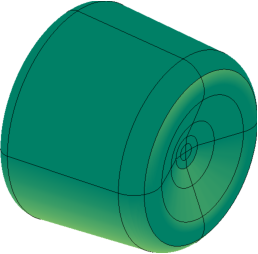
\includegraphics[width=0.4\textwidth]{electrode.pdf}
   \end{center}
\end{posterboxenv}

\begin{posterboxenv}[title=Isogeometric Analysis]{name=iga, row=2, span=1}
   \begin{tikzpicture}
      \draw (0,0) grid (10,10);
      \draw (2,5) .. controls (4,7) .. (7,3);
   \end{tikzpicture}
   introduce nurbs, show 2d geometry with control mesh, mention iga as FEA method with nurbs basis functions
\end{posterboxenv}

\begin{posterboxenv}[title=Geometry Optimization]{name=geo, column=2, row=1, span=1}
   % \begin{center}
      \begin{tikzpicture}
\begin{axis}[
   scale only axis = true,
   width = 0.45\textwidth,
   axis equal,
   try min ticks=4,
   max space between ticks=1000pt,
   enlargelimits=true,
   x unit=m,
   y unit=m]

   \addplot[color=brewergrey] table {figures/200kV/nurbs/nurbs_5_1.dat};
   \addplot[color=brewerred, mark=*] table {figures/200kV/nurbs/nurbs_5_1_coefs.dat};
   \addplot[color=brewergrey, dashed] table {figures/200kV/nurbs/nurbs_5_1_net.dat};

   \addplot[color=brewergrey] table {figures/200kV/nurbs/nurbs_6_3.dat};
   \addplot[color=brewerred, mark=*] table {figures/200kV/nurbs/nurbs_6_3_coefs.dat};
   \addplot[color=brewergrey, dashed] table {figures/200kV/nurbs/nurbs_6_3_net.dat};

   \addplot[color=brewergrey] table {figures/200kV/nurbs/nurbs_7_3.dat};
   \addplot[color=brewerred, mark=*] table {figures/200kV/nurbs/nurbs_7_3_coefs.dat};
   \addplot[color=brewergrey, dashed] table {figures/200kV/nurbs/nurbs_7_3_net.dat};

   \addplot[color=brewergrey] table {figures/200kV/nurbs/nurbs_8_3.dat};
   \addplot[color=brewerred, mark=*] table {figures/200kV/nurbs/nurbs_8_3_coefs.dat};
   \addplot[color=brewergrey, dashed] table {figures/200kV/nurbs/nurbs_8_3_net.dat};

   \addplot[color=brewergrey] table {figures/200kV/nurbs/nurbs_9_3.dat};
   \addplot[color=brewerred, mark=*] table {figures/200kV/nurbs/nurbs_9_3_coefs.dat};
   \addplot[color=brewergrey, dashed] table {figures/200kV/nurbs/nurbs_9_3_net.dat};

   \addplot[color=brewergrey] table {figures/200kV/nurbs/nurbs_10_2.dat};
   \addplot[color=brewerred, mark=*] table {figures/200kV/nurbs/nurbs_10_2_coefs.dat};
   \addplot[color=brewergrey, dashed] table {figures/200kV/nurbs/nurbs_10_2_net.dat};

   \addplot[color=brewergrey] table {figures/200kV/nurbs/nurbs_11_2.dat};
   \addplot[color=brewerred, mark=*] table {figures/200kV/nurbs/nurbs_11_2_coefs.dat};
   \addplot[color=brewergrey, dashed] table {figures/200kV/nurbs/nurbs_11_2_net.dat};
\end{axis}
\end{tikzpicture}

      \begin{tikzpicture}[scale=1]
\begin{axis}[
   scale only axis = true,
   width = 0.45\textwidth,
   axis equal,
   try min ticks=4,
   max space between ticks=1000pt,
   enlargelimits=true,
   x unit=m,
   y unit=m,
   hide axis]

   \addplot[color=black] table {nurbs-opt/nurbs_5_1.dat};
   \addplot[color=TUDa-9a, mark=*, only marks] table {nurbs-opt/nurbs_5_1_coefs.dat};
   \addplot[color=TUDa-0b, dashed] table {nurbs-opt/nurbs_5_1_net.dat};

   \addplot[color=black] table {nurbs-opt/nurbs_6_3.dat};
   \addplot[color=TUDa-9a, mark=*, only marks] table {nurbs-opt/nurbs_6_3_coefs.dat};
   \addplot[color=TUDa-0b, dashed] table {nurbs-opt/nurbs_6_3_net.dat};

   \addplot[color=black] table {nurbs-opt/nurbs_7_3.dat};
   \addplot[color=TUDa-9a, mark=*, only marks] table {nurbs-opt/nurbs_7_3_coefs.dat};
   \addplot[color=TUDa-0b, dashed] table {nurbs-opt/nurbs_7_3_net.dat};

   \addplot[color=black] table {nurbs-opt/nurbs_8_3.dat};
   \addplot[color=TUDa-9a, mark=*, only marks] table {nurbs-opt/nurbs_8_3_coefs.dat};
   \addplot[color=TUDa-0b, dashed] table {nurbs-opt/nurbs_8_3_net.dat};

   \addplot[color=black] table {nurbs-opt/nurbs_9_2.dat};
   \addplot[color=TUDa-9a, mark=*, only marks] table {nurbs-opt/nurbs_9_2_coefs.dat};
   \addplot[color=TUDa-0b, dashed] table {nurbs-opt/nurbs_9_2_net.dat};
\end{axis}
\end{tikzpicture}

   % \end{center}
   state optimization problem, show C1 nurbs that is optimized
\end{posterboxenv}


\begin{posterboxenv}[title=Results]{name=res, column=2, row=2}
   show field magnitude for starting and optimized geometry (also values?)
\end{posterboxenv}

\end{tcbposter}

\end{document}
